\chapter{Nền tảng lý thuyết}
\section{Kiến thức nền tảng}
Trong phần này chúng ta sẽ đi vào việc ôn tập, nhắc lại một số định nghĩa, kiến
thức của các môn nền tảng về Xác suất thống kê, Giải tích và Đại số tuyến tính.
Đó là các kiến thức tối quan trọng được sử dụng rất nhiều trong việc xây dựng
cũng như tối ưu thuật toán trong Machine Learning \cite{MachineLearningLec, MachineLearningSec}. \\\\  
Sau đó, chúng ta sẽ đi đến trình bày các kiến thức vận dụng chính yếu về 
Machine Learning và Kinh tế, nó được sử dụng để xây dựng nên mô hình phương 
pháp giải quyết vấn đề phân lớp.
\subsection{Đại số tuyến tính}
\begin{itemize}
\item Ma trận A cấp $m \times n$ là một mảng hình chữ nhật gồm m hàng và n cột
với các phần tử là số hoặc các đối tượng toán học được biễu diễn như sau:\\
\[
\begin{bmatrix}
    a_{11} & \dots  & a_{1n} \\
    \vdots & \ddots & \vdots \\
    a_{m1} & \dots  & a_{mn}
\end{bmatrix}
= (a_{ij}),\: \forall\: i = \overline{1,m},\: j = \overline{1,n}
\]
Trong đó:\\
\tab $a_{ij} \in R$: là phần tử thuộc dòng i và cột j của ma trận A.\\
\tab $m$: số dòng của ma trận A. \\
\tab $n$: số cột của ma trận A.\\ 
Ký hiệu $M_{m \times n}$ là tập hợp các ma trận $m \times n$.\\ 
\item Vector là một ma trận $A_{m1}$ có một cột và m dòng.
\[
A = 
\begin{bmatrix}
a_{11}\\
\vdots\\
a_{m1}
\end{bmatrix}
\]
\item Phép cộng và phép trừ hai ma trận. Để cộng và trừ hai ma trận ta thực hiện
việc cộng và trừ lần lượt cho từng phần tử tương ứng nhau của hai ma trận. Lưu ý, hai
ma trận cần có cùng chiều, nghĩa là số hàng và số cột của hai ma trận là như
nhau.\\
\[
\begin{bmatrix}
a & b\\
c & d
\end{bmatrix}
+
\begin{bmatrix}
w & x\\
y & z
\end{bmatrix}
=
\begin{bmatrix}
a+w & b+x\\
c+y & d+z
\end{bmatrix}
\]
\item Phép nhân vô hướng là phép nhân giữa một ma trận và một số, ta thực hiện
phép nhân vô hướng bằng cách nhân số đó cho tất cả các phần tử trong ma trận.\\
\[
\begin{bmatrix}
a & b\\
c & d
\end{bmatrix}
\times x =
\begin{bmatrix}
a\times x & b\times x\\
c\times x & d\times x
\end{bmatrix}
\]
\item Nhân hai ma trận: Cho $A \in M_{m\times k}$ và $B \in M_{k\times n}$. Gọi
$A_1, A_2, \dots,A_m$ là m dòng của A; $B^{(1)}, B^{(2)}, \dots, B^{(n)} $ là n cột
của B.\\
Ta viết:
\[
A = 
\begin{bmatrix}
A_{1}\\
\vdots\\
 A_{m}
\end{bmatrix} ;\quad
B = 
\begin{bmatrix}
B^{(1)} & \dots & B^{(n)}
\end{bmatrix}
\]\\
Với 
\[
A_i = 
\begin{bmatrix}
a_{i1} & a_{i2} & \dots & a_{ik}
\end{bmatrix} ;\quad
B^{(j)} = 
\begin{bmatrix}
b_{1j}\\ b_{2j} \\ \vdots \\ b_{kj}
\end{bmatrix}
\]\\
Khi đó $C=A\times B$ gọi là ma trận tích của A với B và phần tử  của $C_{ij}$
được xác định như sau:
$c_{ij} = A_i \times B^{(j)} = a_{i1}b_{1j} + a_{i2}b_{2j} + \dots +
a_{ik}b_{kj}$
Một số tính chất của phép nhân hai ma trận:
\begin{itemize}
  \item Không có tính giao hoán: $A \times B \neq B \times A$
  \item Tính kết hợp: $(A\times B) \times C = A\times (B\times C)$
\end{itemize}
\item Ma trận đảo của A được ký hiệu là $A^{-1}$ với tích của hai ma trận là một
ma trận đơn vị.
\item Ma trận chuyển vị của ma trận A là ma trận có được từ A bằng cách viết các
hàng của ma trận A theo thứ tự thành cột, ký hiệu là $A^T$.
\[
A = 
\begin{bmatrix}
a & b\\
c & d\\
e & f
\end{bmatrix}
\Rightarrow A^T =
\begin{bmatrix}
a & c & e\\
b & d & f
\end{bmatrix}
\]
\item Ma trận đối xứng: Gọi $a_{ij}$  là phần tử của ma trận đối xứng A, thì
$\forall\:i,j:\:a_{ij} = a_{ji}$\\
Tính chất liên quan: Gọi x là một vector n chiều $(n \times 1)$ và $A=x.x^T$
thì A là một ma trận đối xứng $(n \times n)$
\item Ma trận bán định dương (positive semi-definite): Ma trận M $(n \times n)$
được định nghĩa là ma trận bán định dương khi vào chỉ khi với vetor V bất kỳ có
n chiều ta luôn có: $V^T MV>0$
\end{itemize}

\subsection{ Đại số tuyến tính mở rộng đối với ma trận}
\begin{itemize}
  \item Phép toán trace: Phép toán trace được ký hiệu là “tr” và nó thực hiện
  phép tính tổng đường chéo của ma trận vuông.
  \[ trA = \sum_{i=1}^{n} A_{ii} \]
  Các tính chất của phép toán trace với A, B, C là ma trận vuông và a là
  hằng số:
  \begin{enumerate}
    \item $trABC = trCAB = trBCA$
    \item $trA = trA^T$
    \item $tr(A+B) = trA + trB$
    \item $tr(a.A) = a.trA$
  \end{enumerate}
  \item Đạo hàm của hằng số theo ma trận (scalar-by-matrix):
  Với ma trận $A (m \times n)$
  \[  A =
  \begin{bmatrix}
  \frac{\partial f}{\partial A_{11}} & \dots & \frac{\partial f}{\partial
  A_{1n}}\\
  \vdots & \ddots & \vdots \\
  \frac{\partial f}{\partial A_{m1}} & \dots & \frac{\partial f}{\partial
  A_{mn}}  
   \end{bmatrix} \]
   Thì 
   \[ \nabla_A f(A) = 
   \begin{bmatrix}
  \frac{\partial f}{\partial A_{11}} & \dots & \frac{\partial f}{\partial
  A_{m1}}\\
  \vdots & \ddots & \vdots \\
  \frac{\partial f}{\partial A_{1n}} & \dots & \frac{\partial f}{\partial
  A_{mn}}  
   \end{bmatrix}  \]
  Ví dụ: Cho ma trận A = $ \begin{bmatrix} A_{11} & A_{12} \\ A_{21} & A_{22}
  \end{bmatrix} $ và $f(A) = A_{11} + 2A_{12}^{2} + 3A_{21}A_{22}$ suy ra
  \[ \nabla_A f(A) = \begin{bmatrix} 1 & 3A_{22} \\ 4A_{12} & 3A_{21}
  \end{bmatrix} \]
  Các tính chất của đạo hàm ma trận với A, B, C là ma trận vuông nxn và x là
  vector n chiều:
  \begin{enumerate}
    \item $\nabla_A trAB = B^T$
    \item $\nabla_{A^T} f(A) = (\nabla_A f(A))^T$
    \item $\nabla_A trABA^TC = CAB + C^TAB^T$
    \item $\nabla_A |A|=|A|(A^{-1})^T$
    \item $\nabla_x (x^TAx) = x^T(A + A^T)$. Nếu ma trận A đối xứng thì
    $\nabla_x (x^TAx) = 2x^TA$
  \end{enumerate}
  \item Eigenvalues và Eigenvectors:
  \[ Av=\lambda v \]
  Trong đó\\
  \tab A là ma trận $(n\times n)$\\
  \tab v là vector n chiều $(n\times 1)$\\
  \tab $\lambda$ là một eigenvalue của A\\
  \tab v là một eigenvector của A\\
  Mệnh đề liên quan:
  \begin{enumerate}
    \item Một ma trận A có thể có nhiều eigenvalue và nhiều eigenvector
    \item Cho các eigenvector của A là $v_1,v_2,\dots,v_n$ không phụ thuộc tuyến
    tính vào nhau, và $\lambda_1,\lambda_2,\dots,\lambda_n$ là các eigenvalue
    tương ứng. Khi đó ta có:
    \[ A = PDP^{-1} \]
    Với:
    \[ P = \begin{bmatrix} v_1 & v_2 & \dots & v_n \end{bmatrix} \]
    \[ D = 
    \begin{bmatrix} 
    \lambda_1 & 0 & \dots & 0 \\
    0 & \lambda_2 & \dots & 0 \\
    \vdots & \vdots & \ddots & \vdots \\
    0 & 0 & \dots & \lambda_n 
    \end{bmatrix} \]
  \end{enumerate}
  \item Ma trận trực giao\\
  Một ma trận A được gọi là trực giao nếu tích của ma trận A và chuyển vị của nó
  là một ma trận đơn vị. Ví dụ
  \[ \begin{bmatrix} 
    1 & 0 & 0 \\
    0 & \frac{3}{5} & -\frac{4}{5} \\
    0 & \frac{4}{5} & \frac{3}{5}
    \end{bmatrix} \]
  \[ AA^T = 
  \begin{bmatrix} 
    1 & 0 & 0 \\
    0 & \frac{3}{5} & -\frac{4}{5} \\
    0 & \frac{4}{5} & \frac{3}{5}
    \end{bmatrix}
    \begin{bmatrix} 
    1 & 0 & 0 \\
    0 & \frac{3}{5} & \frac{4}{5} \\
    0 & -\frac{4}{5} & \frac{3}{5}
    \end{bmatrix} = 
    \begin{bmatrix} 
    1 & 0 & 0 \\
    0 & 1 & 0 \\
    0 & 0 & 1
    \end{bmatrix}
     \]
     \item Ma trận đường chéo\\
     Ma trận đường chéo là ma trận có các giá trị $a_{ij} = 0$ nếu $i \neq j$ và
     các giá trị còn lại của ma trận là khác 0
     \[\begin{bmatrix} 
    a_{11} & 0 & \dots & 0 \\
    0 &  a_{22} & \dots & 0 \\
    \vdots & \vdots & \ddots & \vdots \\
    0 & 0 &  \dots & a_{nn}
    \end{bmatrix}
     \]
\end{itemize}

\subsection{Xác suất thống kê}
\begin{itemize}
  \item Xác suất có điều kiện: Cho hai biến cố A và B. Ta gọi xác suất của biến
  cố A khi biến cố B đã xảy ra là xác suất của A với điều kiện B, ký hiệu là P(A|B).
  \item Công thức xác suất đầy đủ: Cho $A_1, A_2, \dots,A_m$ là nhóm đầy đủ các
  biến cố, với mọi biến cố F ta có:\\
  \[
  P(F) = P(A_1).P(F|A_1) + P(A_2).P(F|A_2) + \dots + P(A_n).P(F|A_n) 
  \]
  \item Công thức Bayes: Cho $A_1, A_2, \dots,A_m$ là nhóm đầy đủ các biến cố,
  với mỗi $k (k = \overline{1,n})$, ta có:
  \[
  P(A_k|F) = \frac{P(A_k).P(F|A_k)}{P(F)} = \frac{P(A_k).P(F|
  A_k)}{\sum_{i=1}^{n} P(A_i).P(F| A_i)}
  \]
  \item Kỳ vọng: Cho X là đại lượng ngẫu nhiên rời rạc có các bảng phân phối xác
  suất.
  \begin{table}[h]
  \centering
  \begin{tabular}{|c|c|c|c|c|c|}
  \hline
  X & $X_1$ & $X_2$ & \dots & $X_n$ & \dots\\
  \hline
  P & $P_1$ & $P_2$ & \dots & $P_n$ & \dots\\
  \hline
  \end{tabular}
  \caption{Bảng phân phối xác suất}
  \end{table}\\
  Khi đó ta gọi kỳ vọng của X là số:
  \[
  E(X) = x_1p_1 + x_2p_2 + \dots + x_np_n + \dots = \sum_{n=1}^{\infty} x_np_n
  \]
  Nếu X là đại lượng ngẫu nhiên liên tục có hàm mật độ f(x) thì kỳ vọng của X
  là:
  \[
  E(X) = \int_{-\infty}^{+\infty} xf(x) dx
  \]
  \item Phương sai: Cho X là một đại lượng ngẫu nhiên có kỳ vọng E(X). Khi đó ta
  ký hiệu phương sai của X là D(X):
  \[ D(X) = E[(X-E(X))^2] \]
  \item Phân phối nhị thức: Đại lượng ngẫu nhiên rời rạc $X={0,1,2,\dots,n}$ gọi
  là có phân phối nhị thức nếu tồn tại số $p \in (0,1)$ sao cho:
  \[ p_k = P(X=k) = C_{n}^{k}p^kq^{n-k},\:q=1-p,\:k=\overline{0,n} \]
  Ta ký hiệu: $X \sim B(n,p)$ 
  \item Phân phối chuẩn: Đại lượng ngẫu nhiên X gọi là có phân phối chuẩn nếu
  hàm mật độ của X có dạng:
  \[ f(x) = \frac{1}{\sigma \sqrt{2\pi}}e^{-\frac{(x-a)^2}{2\sigma^2}},\:\sigma
  > 0
  \]
  Ta ký hiệu: $X \sim \mathcal{N}(a,\sigma^2)$
  \item Phân phối chuẩn tắc: Đại lượng : $X \sim \mathcal{N}(0,1)$ gọi là
  có phân phối chuẩn tắc. Nếu X có phân phối chuẩn tắc thì hàm mật độ của X là:
  \[ f(x)=\frac{1}{\sqrt{2\pi}}e^{-\frac{x^2}{2}} \]
  \item Phân phối Gaussian: Phân phối chuẩn với n chiều còn được gọi với tên
  khác là phân phối Gaussian, nó được tổng quát hóa từ phân phối chuẩn của số
  thực lên cho vector nhiều chiều. Phân phối này được tham số hóa bằng hai đại
  lượng: một vector trung bình $\mu \in R^n$ và một ma trận tương quan
  (Covariance matrix) $\Sigma \in R^{n \times n}$ với $\Sigma \geq 0$ là một ma
  trận đối xứng (symmetric) và bán định dương (positive semi-definite). Ký hiệu:
  $\mathcal{N} (\mu, \Sigma)$.\\
  Ta định nghĩa, một vector x có quy luật phân phối chuẩn $\mathcal{N} (\mu,
  \Sigma)$ khi và chỉ khi hàm mật độ của X được biểu diễn dưới dạng:
  \[ p(x;\mu,\Sigma) = \frac{1}{(2\pi)^{n/2}|\Sigma|^{1/2}} exp\left(
  -\frac{1}{2}(x-\mu)^T\Sigma^{-1}(x-\mu) \right) \] Từ đó ta suy ra kỳ vọng của
  vector X chính là $\mu$:
  \[ E[X] = \int_x xp(x;\mu,\Sigma)dx = \mu \]
  Tổng quát hóa Covariance của một biến giá trị thực ngẫu nhiên ta có Covariance
  của một biến giá trị vector ngẫu nhiên và được định nghĩa:
  \[ Cov(Z) = E[(Z-E[Z])(Z-E[Z]^T)] = E[Z.Z^T] - (E[Z])(E[Z])^T \]
  Mặc khác, nếu $X \sim \mathcal{N}(\mu,\Sigma)$ thì: 
  \[ Cov(X) = \Sigma \]
  \item Relative Difference Percentage: Cho bộ số $\{ x_1, x_2,..., x_n \}$ khi đó
  \[
    RDP_i(n)=\frac{x_n-x_{n-i}}{x_{n-i}}
  \]
\end{itemize}

\section{Kinh tế}
Vì luận văn này đang giải quyết một bài toán về kinh tế nên để hiểu được công 
việc, ta cần nắm được các ý niệm cơ bản về kinh tế.
\subsection{Phiên giao dịch và các giá trị cơ bản}
Gọi T là một mốc thời gian bất kỳ, P là khoảng thời gian được chọn là một phiên 
giao dịch. Ta có thể nói một cách đơn giản là phiên giao dịch được mở tại thời 
điểm T và được kết thúc tại thời điểm T + P.\\\\
Cụ thể, giả sử chọn mốc mở phiên là 9:00 am và phiên giao dịch có thời hạn là 
30 phút, điều đó có nghĩa là kết thúc phiên giao dịch sẽ là 9:30 am.\\\\
Ngoài ra:
\begin{itemize}
\item Giá mở phiên: là giá bán của một giao dịch gần nhất sau thời điểm T. Ví dụ tại thời 
điểm 9:01 am có một giao dịch bán 1 BTC là \$779 và trong khoảng thời gian 9:00 am 
đến 9:01 am không hề có bất kỳ giao dịch nào khác ngoại trừ giao dịch này, thì ta có thể 
nói giá mở phiên sẽ là \$779.
\item Giá đóng phiên: là giá bán của một giao dịch gần nhất trước thời điểm T + P.
\item Giá phiên cao nhất: là giá bán cao nhất của một giao dịch trong khoảng thời gian diễn ra phiên 
giao dịch, cụ thể là từ thời điểm T đến thời điểm T + P. Ví dụ, trong khoảng thời gian 9:00 am (thời điểm 
mở phiên) đến thời gian 9:30 am (thời điểm đóng phiên) có một giao dịch BTC với giá là 
\$801 và là giao dịch có giá trị cao nhất. Vậy ta có thể nó giá phiên cao nhất là 
\$801.
\item Giá phiên thấp nhất: là giá bán thấp nhất của một giao dịch trong khoảng thời gian diễn ra phiên 
giao dịch, cụ thể là từ thời điểm T đến thời điểm T + P.
\item Lượng giao dịch: số lượng BTC chênh lệch giữa giá phiên cao nhất và giá phiên 
thấp nhất của một phiên giao dịch.
\item Trung bình giao dịch: giá trị USD trung bình của tất cả các giao dịch diễn 
ra trong khoảng thời gian một phiên giao dịch.
\end{itemize}
\subsection{Rate of Change}
Đại lượng đo sự khác nhau của giá tại phiên thứ x so với n phiên trước đó. 
Giá sử $P(x)$ là giá của phiên thứ $x$ thì:
\[ ROC_{n}(x)=\frac{P(x)-P(x-n)}{P(x-n)}\]
Nếu $ROC > 0$ thì giá thị trường đang có xu hướng đi lên (tăng giá).
Ngược lại, với $ROC < 0$ thì giá thị trường đang có xu hướng giảm xuống.
\subsection{Stochastic Oscillator}
Đại lượng dùng để đo xu hướng mua/bán của thị trường tại thời điểm phiên x thông 
qua n phiên trước đó. Giả sử:\\\\
\tab $L_{n} = $ giá phiên thấp nhất trong n phiên\\
\tab $H_{n} = $ giá phiên cao nhất trong n phiên\\
\tab $P(x) = $ giá của ngày x\\
\[\%K=\frac{P(x)-L_{n}}{H_{n}-L_{n}}\]
Nếu $ \%K $ nhỏ hơn 20 thì thị trường đang có xu hướng mua vào và nếu lớn hơn 
80 thì thị trường đang có xu hướng bán ra.


\section{Machine Learning}

\subsection{Khái niệm cơ bản}
\subsubsection{Machine Learning}
Machine Learning có hai cách định nghĩa chính và đang được chấp nhận phổ biến:
\begin{itemize}
  \item Theo Arthur Samuel: \textit{``Là một lĩnh vực nghiên cứu mà nó cung cấp cho
  máy tính khả năng học hỏi mà không cần lập trình một cách tường minh.''}
  \item Theo Tom Mitchell: \textit{``Một chương trình máy tính được chấp nhận
  là học hỏi được kinh nghiệm E bằng cách thực hiện một vài tác vụ T theo phép đo hiệu
  năng P, nếu và chỉ nếu việc thực thi các tác vụ trong T được đo bởi phép đo P
  đem lại kết quả là kinh nghiệm E được cải thiện.''}
\end{itemize}
\subsubsection{Supervised Learning - Học có giám sát}
Chúng ta được cho một tập dữ liệu đã biết với các input và output tương ứng
nhau. Ý tưởng là chúng ta sẽ đi tìm mối quan hệ giữa input và output đó chính là
Supervised Learning.\\\\
Vấn đề của Supervised Learning được phân loại thành hai
vấn đề chính là “Regression” và “Classification”. Trong vấn đề “Regression”,
chúng ta sẽ cố gắng dự đoán kết quả output tiếp theo một cách liên tục, nghĩa là
chúng ta đi tìm ra một hàm đầu ra liên tục tổng quát với biến là các thuộc tính
đầu vào. Còn với vấn đề “Classification”, chúng ta thay vì cố gắng dự đoán kết
quả liên tục thì ta sẽ đi dự đoán chúng theo hướng rời rạc, hiểu theo một cách
khác là chúng ta đi tìm một phép phân loại rời rạc cho output với các biến
input.
\subsubsection{Unsupervised Learning - Học không giám sát}
Học không giám sát cho phép chúng ta tiếp cận các vấn đề mà ta chưa hề hoặc biết
rất ít kết quả của chúng ta sẽ trông như thế nào. Chúng ta có thể xây dựng cấu
trúc của dữ liệu mà không cần thiết phải biết ảnh hưởng của các biến đó.\\\\
Chúng ta thực hiện việc này dựa trên ý tưởng gom cụm dữ liệu bằng cách xem xét
mối quan hệ giữa các thuộc tính của dữ liệu. Các hướng tiếp cận dựa trên nhưng 
phương pháp như vậy thường được gọi là “Clustering”.

\subsection{Thông số đánh giá}
Có ba tham số cơ bản dùng để xem xét và đánh giá giải thuật trong Machine Learning.
Gọi:
\begin{itemize}
\item True positive là TP
\item False positive là FP
\item True negative là TN
\item False negative là FN
\end{itemize}
Thì:\\
\[
  Accuracy = \frac{TP+TN}{TP+FP+TN+FN}
\]
\[
  Precision = \frac{TP}{TP+FP}
\]
\[
  Recall = \frac{TP}{TP+FN}
\]\\
\begin{figure}[h!]
\centering
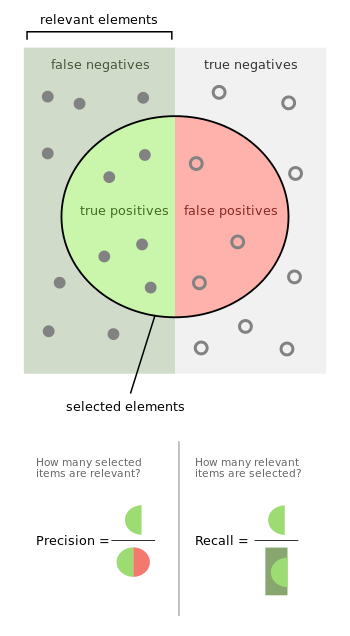
\includegraphics[height=7in, keepaspectratio=true]{precision_recall.png}
\caption{Validation Parameters}
\end{figure}\\
\subsection{Neural Network - Deep Learning}
Deep Learning nói chung và Neural Network nói riêng là hai phạm trù xuất hiện 
không lâu đối với Machine Learning, đại diện cho hướng tiếp cận gần với 
cái nhìn thực tế, học nhiều cấp và học từ bản chất dữ liệu. Deep Learning 
thường giải quyết rất tốt với các loại dữ liệu mang tính ``con người'' như 
hình ảnh, âm thanh ... \cite{NeuralNetworksandDeepLearning} 
\subsubsection{Ý tưởng giải thuật}
Bộ não con người là một trong những phát minh vĩ đại nhất của tự nhiên, nó 
có thể giải quyết các bài toán mà đối với máy tính là cực kỳ phức tạp chỉ trong 
vài giây hoặc kể cả là vài phần giây, các khả năng phán đoán, học hỏi, tích lũy 
kinh nghiệm đó chính là điều tuyệt diệu của bộ não con người. Và các nhà khoa học 
khao khát một thứ gì đó trong giới máy tính có khả năng như vậy.\\\\
Dựa trên ý tưởng kết cấu của bộ não gồm hàng tỷ neural liên kết lại với nhau, 
mỗi neural chỉ đưa ra một tín hiệu hết sức đơn giản, nhưng khi hàng tỷ neural liên kết 
hình thành nên một hệ thống phức tạp thì từ đó có khả năng giải quyết các vấn đề 
phức tạp. Các nhà khoa học máy tính, đã cố gắng định nghĩa một neural đơn lẻ 
trong phạm trù máy tính và được gọi là perceptron, từ đó kết nối lại với nhau 
để tạo nên một hệ thống hữu hạn các perceptron có khả năng giả lập một bộ não 
người - mạng neural nhân tạo.

\subsubsection{Cấu trúc một Perceptron}
Một perceptron sẽ có các input $x_1, x_2, ...$ và output sẽ là một giá trị 
nhị phân.\\
\begin{figure}[h!]
\centering
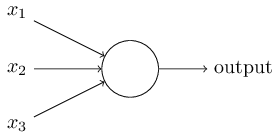
\includegraphics[height=1.5in, keepaspectratio=true]{perceptron.png}
\caption{Multilayer Neural Network}
\end{figure}\\
Một ví dụ đơn giản dựa vào hình trên, ta thấy perceptron này có 3 input là 
$x_1, x_2, x_3$ , giả sử đi kèm với mỗi input sẽ có một giá trị trọng 
số $w_1, w_2, w_3$. Output được định nghĩa là 0 và 1, nhận giá trị 0 
khi $\sum_j w_j x_j$ nhỏ hơn giá trị ngưỡng và 1 khi lớn gơn giá trị ngưỡng.\\\\
Biểu diễn đại số:\\
\[
  output = 
  \bigg\{
    _{0 \quad if \, \sum_j w_j x_j \, \leq \, threshold}
    ^{1 \quad if \, \sum_j w_j x_j \, > \, threshold}
\]
Các hàm số như trên được gọi là activation function, có nhiều loại activation
 function khác nhau như: $sigmoid , tang ...$ 

\subsubsection{Multilayer Neural Network}
Hiển nhiên, một perceptron không thể mô phỏng nên được một bộ não người, để 
có thể đưa ra một quyết định tương tự như bộ não người các perceptron này cần 
được kết nối với nhau thành một mạng lưới - Multilayer Neural Network.\\
\begin{figure}[h!]
\centering
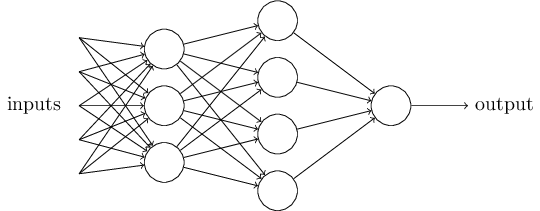
\includegraphics[height=2in, keepaspectratio=true]{multilayerneuralnetwork.png}
\caption{Perceptron}
\end{figure}\\
Multilayer Neural Network được cấu thành bằng cách sắp xếp các perceptron thành 
từng lớp. Các perceptron ở mỗi lớp sẽ kết nối với tất cả các perceptron ở các 
lớp liền kề, cột những perceptron đầu tiên được gọi là input layer, chúng có 
chức năng tiếp nhận các input để cho ra các output. Các output ở lớp trước sẽ chính là 
input cho các perceptron ở lớp tiếp theo. Các perceptron ở lớp cuối cùng được gọi là 
output layer, trong trường hợp này đặc biệt chỉ có duy nhất một perceptron. Còn 
lại các lớp perceptron khác được gọi là hidden layer.\\\\
Giả sử input của perceptron là $x_1, x_2, ...$ tương ứng là đó là các trọng 
số $w_1, w_2, ...$. Thêm vào đó định nghĩa về bias, ở đây bias là một giá trị 
đại diện độ lệch của từng perceptron và được ký hiệu $b_1, b_2, ...$. Ta có biểu diễn của activation 
function:\\
\[
  output = 
  \bigg\{
    _{0 \quad if \, \sum_j w_j x_j + b_i\, \leq \, 0}
    ^{1 \quad if \, \sum_j w_j x_j + b_i\, > \, 1}
\]
Ví dụ:\\
\begin{figure}[h!]
\centering
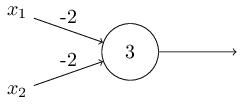
\includegraphics[height=1in, keepaspectratio=true]{exmln.png}
\caption{Perceptron with Bias example}
\end{figure}\\
Ta có $w_1=w_2=-2$ và $b=3$, khi đó nếu input $x_1=1,\, x_2=0$ suy ra $ 
w_1*x_1+w_2*x_2+b=(-2)*1+(-2)*0+3=1$, ta có thể chọn $threshold=0$ vì $1>0$
nên $output=1$.

\subsubsection{Sigmoid Function - Hàm Sigmoid}
Với dạng activation function được định nghĩa ở trên, giá trị của activation 
function gần như không có giới hạn. Vậy tại sao việc không có giới hạn lại 
cần được quan tâm. Trong một trường hợp cụ thể, với việc sử dụng activation 
function như trên có thể dẫn đến trường hợp đầu ra của một perceptron sẽ nhận 
giá trị rất lớn - giả sử là 1000, những một perceptron khác sẽ nhận giá trị rất 
bé - giả sử 0.001. Vì thế khi đến lớp tiếp theo thì gần như perceptron cho kết 
quả đầu ra là giá trị bé sẽ mất đi độ ảnh hưởng và làm mất cân đối cho toàn mạng.\\\\
Do đó để giới hạn giá trị của activation function chúng ta sẽ sử dụng hàm sigmoid. 
Sigmoid function được định nghĩa như sau:\\
\[
  \sigma(z)=\frac{1}{1+e^{-z}}
\]
Áp dụng Sigmoid function vào activation function ta có activation function dạng
sigmoid và khi đó activation function của chúng ta sẽ có dạng:\\
\[
  \frac{1}{1+exp(-\sum_j w_j x_j -b)}
\]
Lúc này ta có một activation function có giá trị được giới hạn trong khoảng 
từ 0 đến 1. Nhưng chú ý, giá trị của activation function là liên tục, để rời 
rạc hóa giá trị của activation function ta có thể sử dụng một phương pháp 
quen thuộc - sử dụng threshold. Điển hình ta chọn threshold = 0.5, nếu lớn hơn 
thì activation function sẽ nhận 1 và ngược lại sẽ nhận 0.\\\\
Để hiểu rõ hơn tại sao chúng ta quan sát hai đồ thị của sigmoid function và 
activation function có dạng sigmoid và đã được rời rạc hóa giá trị:\\
\begin{figure}[h!]
\centering
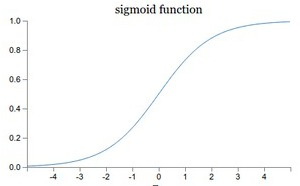
\includegraphics[height=2.5in, keepaspectratio=true]{sigmoid.jpg}
\caption{Sigmoid Function}
\end{figure}\\
\begin{figure}[h!]
\centering
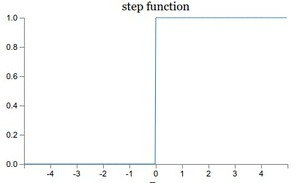
\includegraphics[height=2.5in, keepaspectratio=true]{step.jpg}
\caption{Step Function}
\end{figure}\\

\subsubsection{Giải thuật Backpropagation}
Sau khi đã có xây dựng thành công một mô hình Multilayer Neural Network, công 
việc cuối cùng là cung cấp khả năng tự học hỏi từ đó để bản thân mạng có thể 
tự xây dựng mô hình và đưa ra các quyết định cụ thể.\\\\
Cụ thể, khi nhìn lại một Multilayer Neural Network với activation function là 
sigmoid function thì các tham sô $w, b$ là chưa biết và việc cung cấp khả năng 
tự học hỏi chính là cung cấp một giải thuật giúp mạng tìm được các tham số 
$w, b$ với một tập kinh nghiệm - hay tập huấn luyện - ${x, y}$ cụ thể, trong 
đó $x$ là input và $y$ là output tương ứng với từng bộ $x$. Giải thuật backpropagation 
là một trong nhưng giải thuật chúng ta cần tìm.\\\\
Trước tiên chúng ta cần đi qua một số ký hiệu:\\\\
\begin{itemize}
\item $w$ là vector của các giá trị trọng số\\ 
\[ w =
\begin{bmatrix}
w_1\\
\vdots\\
w_n
\end{bmatrix}
\]
\item $b$ là vector của các giá trị bias\\ 
\[ b =
\begin{bmatrix}
b_1\\
\vdots\\
b_m
\end{bmatrix}
\]
\item $\sigma$ là sigmoid function
\item $a(\sigma)$ là activation function có dạng sigmoid
\end{itemize}
Biểu diễn activation function:\\
\begin{figure}[h!]
\centering
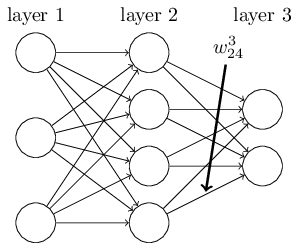
\includegraphics[height=2in, keepaspectratio=true]{exw.png}
\caption{Weight Notation example}
\end{figure}\\
Ví dụ như hình trên, trọng số xuất phát từ perceptron thứ 4 thuộc layer thứ 
2 và kết thúc tại perceptron thứ 2 thuộc layer thứ 3 được ký hiệu là 
$w_{24}^3$.\\\\
Tương tự như vậy với bias và activation function của perceptron thứ j thuộc layer 
thứ l của mạng sẽ được kí hiệu thứ tự là $b_j^l,\,a_j^l$. Ví dụ, bias của perceptron 
thứ 3 thuộc layer thứ 2 sẽ là $b_3^2$ và activation function của perceptron thứ 
1 thuộc layer thứ 3 sẽ là $a_1^3$.\\
\begin{figure}[h!]
\centering
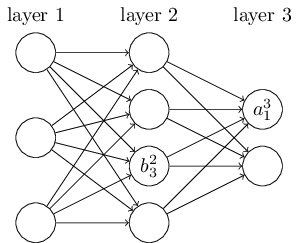
\includegraphics[height=2in, keepaspectratio=true]{exb.png}
\caption{Bias Notation example}
\end{figure}\\
Lúc này ta có biểu diễn toán học đầy đủ của activation function:\\
\[
  a_j^l=\sigma(\sum_k w_{jk}^l a_k^l-1 + b_j^l)
\]
Với ký hiệu vector ta có thể tổng quát phát biểu với dạng:\\
\[
  a^l=\sigma(w^l a^{l-1} + b^l)
\]
\textbf{Cost function:} Trước khi đi vào hiểu được backpropagation có thể làm gì, 
chúng ta cần phải biết một định nghĩa cost function. Vậy cost function là gì? 
Đúng theo tên của hàm, nó dùng để đo lường chi phí của thuật toán. Chi tiết:\\
\[
  C=\frac{1}{2n}\sum_x\|y(x)-a^L(x)\|^2
\]
Ta có thể thấy, dạng hàm số trên hết sức quen thuộc với định nghĩa độ lệch chuẩn 
trong xác suất thống kê nhưng đã được biến đổi một chút. Thay vì giá trị kỳ vọng 
và các điểm xác suất, cost function sử dụng giá trị thực tế $y$ của tập dữ liệu 
và giá trị $y=a$ là giá trị $y$ tính toán được từ $x$ với $w$ và $b$. Vậy ta 
có thể hiểu được, cost function tính toán độ sai lệch của giá trị $a$ so với 
$y$ kỳ vọng thực tế. Do đó, cost function càng nhỏ thì biểu diễn giá trị của 
Multilayer Neural Network sẽ càng gần với thực tế.\\\\
Để tìm được giá trị cực tiểu cho cost function ta sẽ thực hiện vòng lặp:\\
\[
  w_ij^{(l)}:=w_ij^{(l)}-\eta\frac{\sigma}{\sigma w_ij^{(l)}}C(w,b)
\]
\[
  b_i^{(l)}:=b_i^{(l)}-\eta\frac{\sigma}{\sigma b_i^{(l)}}C(w,b)
\]

Trong đó $\eta$ là learning rate - tỉ lệ học, việc hội tụ về giá trị cực tiểu với 
tốc độ và độ chính xác phụ thuộc vào tỉ lệ này.\\\\
Vậy, đi qua một quá trình tìm hiểu về Multilayer Neural Network, ta có thể hiểu 
được việc học hỏi kinh nghiệm của mạng cốt lõi vẫn là việc tìm ra bộ $w$ và $b$ 
tương ứng với ${x, y}$ của bộ dữ liệu luyện tập, và để tìm ra được $w$ và $b$ 
ta có thể sử dụng giải thuật backpropagation.